\section{Length of a vector}

\begin{outcome}
  \begin{enumerate}
    \item Compute the distance between points in $n$-dimensional space.
    \item Compute the length of a vector algebraically and geometrically.
    \item Find vectors that are a given distance from other vectors.
    \item Use algebraic properties of the length operation to prove
      equalities.
    \item Normalize a vector.
\end{enumerate}
\end{outcome}

In this section, we explore what is meant by the length of a vector in
$\R^n$.  We develop this concept by first looking at the distance
between two points in $\R^n$. Consider two points $P=(p_1,p_2)$ and
$Q=(q_1,q_2)$ in the plane, as in the following picture.
\begin{equation*}
  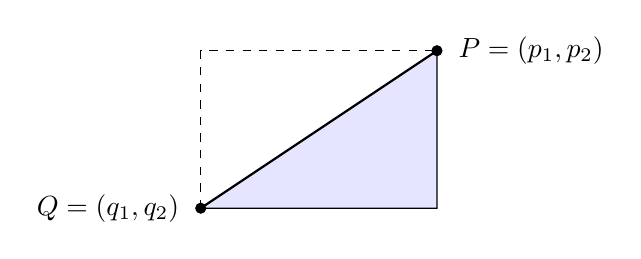
\begin{tikzpicture}[scale=1]
    \draw[dashed] (0,0) -- (0,2) -- (3,2);
    \draw[fill=blue!10] (0,0) -- (3,0) -- (3,2) -- cycle;
    \draw[thick] (0,0) -- (3,2);
    \draw[fill](0,0) circle [radius=1.8pt] node[left=1ex]{$Q=(q_1,q_2)$};
    \draw[fill](3,2) circle [radius=1.8pt] node[right=1ex]{$P=(p_1,p_2)$};
  \end{tikzpicture}
\end{equation*}
The distance between $P$ and $Q$ is shown in the picture as a solid
line, which is the hypotenuse of a right triangle.  The lengths of the
two other sides of this triangle are $\abs{p_{1}-q_{1}} $ and
$\abs{p_{2}-q_{2}}$. Therefore, the Pythagorean Theorem implies the
length of the hypotenuse (and thus the distance between $P$ and $Q$)
equals
\begin{equation*}
  d(P,Q)
  =\sqrt{\abs{p_{1}-q_{1}}^{2}+\abs{p_{2}-q_{2}}^{2}}
  =\sqrt{(p_{1}-q_{1})^{2}+(p_{2}-q_{2})^{2}}.
\end{equation*}
Now consider two points $P=(p_{1},p_{2},p_{3})$ and
$Q = (q_{1},q_{2},q_{3})$ in 3-dimensional space.
\begin{equation*}
  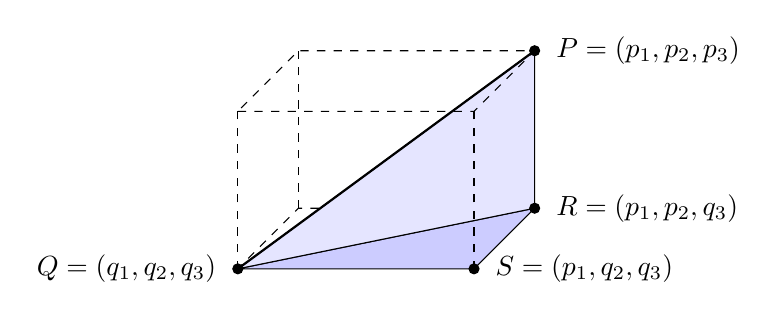
\begin{tikzpicture}[scale=1]
    \draw[dashed] (3,0,-2) -- (0,0,-2) -- (0,0,0);
    \draw[dashed] (0,0,0) -- (0,2,0);
    \draw[dashed] (0,0,-2) -- (0,2,-2);
    \draw[fill=blue!20] (0,0,0) -- (3,0,0) -- (3,0,-2) -- cycle;
    \draw[fill=blue!10] (0,0,0) -- (3,0,-2) -- (3,2,-2) -- cycle;
    \draw[dashed] (0,2,0) -- (3,2,0) -- (3,2,-2) -- (0,2,-2) -- cycle;
    \draw[dashed] (3,0,0) -- (3,2,0);
    \draw[thick] (0,0,0) -- (3,2,-2);
    \draw[fill](0,0,0) circle [radius=1.8pt] node[left=1ex]{$Q=(q_1,q_2,q_3)$};
    \draw[fill](3,2,-2) circle [radius=1.8pt] node[right=1ex]{$P=(p_1,p_2,p_3)$};
    \draw[fill](3,0,-2) circle [radius=1.8pt] node[right=1ex]{$R=(p_1,p_2,q_3)$};
    \draw[fill](3,0,0) circle [radius=1.8pt] node[right=1ex]{$S=(p_1,q_2,q_3)$};
  \end{tikzpicture}
\end{equation*}
We will use the Pythagorean Theorem twice to find the length of the
solid line connecting $P$ and $Q$. First, by the Pythagorean Theorem
applied to the right triangle $QSR$, the length of the line joining
$R$ and $Q$ equals
\begin{equation*}
d(R,Q) = \sqrt{ (p_{1}-q_{1}) ^{2}+(p_{2}-q_{2}) ^{2}}.
\end{equation*}
Second, by the Pythagorean Theorem applied to the triangle $QRP$, the
length of the line joining $P$ and $Q$ equals
\begin{equation*}
d(P,Q)=\sqrt{d(R,Q)^{2}+(p_{3}-q_{3})^{2}}
 =\sqrt{ (p_{1}-q_{1})^{2}+(p_{2}-q_{2})^{2}+(p_{3}-q_{3})^{2}}
\end{equation*}
This discussion motivates the following definition for the distance
between points in $\R^n$.

\begin{definition}{Distance between points}{distance-between-points}
  Let $P=(p_{1},\ldots,p_{n})$ and $Q=(q_{1},\ldots,q_{n})$ be
  two points in $\R^{n}$. Then the
  \textbf{distance}\index{distance!point to point}
  between these points is defined as
  \begin{equation*}
    d(P, Q) = \sqrt{(p_1-q_1)^2 + \ldots + (p_n-q_n)^2}.
  \end{equation*}
  This formula is also called the \textbf{distance
    formula}\index{distance formula}. We may also write $\abs{PQ}$
  for the distance between $P$ and $Q$.
\end{definition}

In the following example, we use
Definition~\ref{def:distance-between-points} to find the distance
between two points in $\R^4$.

\begin{example}{Distance between points}{distance-between-points}
  Find the distance between the points $P=(1,2,-4,6)$ and
  $Q=(2,3,-1,0)$ in $\R^{4}$.
\end{example}

\begin{solution}
  Using the distance formula, we have
  \begin{equation*}
    d(P,Q)= \sqrt{ (1-2) ^{2}+(2-3)
      ^{2}+(-4-(-1)) ^{2}+(6-0)^{2}} =
    \sqrt{1^2+1^2+3^2+6^2} = \sqrt{47}.
  \end{equation*}
\end{solution}

\begin{example}{The plane between two points}{plane-between-two-points}
  Describe the points in $\R^3$ that are equally distant from the two
  points $Q=(1,2,3) $ and $R=(0,1,2)$.
\end{example}

\begin{solution}
  Let $P = (p_1,p_2,p_3)$ be such a point. Then $P$ is the same
  distance from $Q$ and $R$, thus $d(P,Q)=d(P,R)$. By the distance
  formula, we have
  \begin{equation*}
    \sqrt{(p_1-1)^{2}+(p_2-2)^{2}+(p_3-3)^{2}}=
    \sqrt{(p_1-0)^{2}+(p_2-1)^{2}+(p_3-2)^{2}}.
  \end{equation*}
  Squaring both sides, we obtain 
  \begin{equation*}
    (p_1 -1) ^{2}+(p_2 -2) ^{2}+(p_3 -3)
    ^{2}=p_1^{2}+(p_2-1) ^{2}+(p_3 -2) ^{2},
  \end{equation*}
  and so
  \begin{equation*}
    \allowbreak (p_1^{2}-2p_1+1)+(p_2^{2}-4p_2+4)+(p_3^{2}-6p_3+9)=p_1^{2}+(p_2^{2}-2p_2+1)+(p_3^{2}-4p_3+4).
  \end{equation*}
  Simplifying, this becomes
  \begin{equation*}
    -2p_1-4p_2-6p_3+14=-2p_2-4p_3+5,
  \end{equation*}
  which can finally be written as 
  \begin{equation}\label{distance-plane}
    2p_1+2p_2+2p_3=9.
  \end{equation}
  Therefore, the points $P = (p_1,p_2,p_3)$ that are the same
  distance from $Q$ and $R$ form a plane whose equation is given by
  \eqref{distance-plane}.
\end{solution}

We can now use our understanding of the distance between two points to
define what is meant by the length of a vector.

\begin{definition}{Length of a vector}{length-of-vector}
  Let
  \begin{equation*}
    \vect{u} = \begin{mymatrix}{c}u_1\\\vdots\\u_n\end{mymatrix}
  \end{equation*}
  be a vector in $\R^n$. Then the
  \textbf{length}\index{vector!length}\index{length of a vector} of
  $\vect{u}$, written $\norm{\vect{u}}$, is given by
  \begin{equation*}
    \norm{\vect{u}} = \sqrt{u_{1}^2 + \ldots + u_{n}^2}.
  \end{equation*}
  The length of a vector is also sometimes called its
  \textbf{magnitude}%
  \index{magnitude!of a vector}%
  \index{vector!magnitude}.
\end{definition}

This definition corresponds to
Definition~\ref{def:distance-between-points}, if we consider the
vector $\vect{u}$ to have its tail at the point
$0 = (0,\ldots,0)$ and its tip at the point
$U = (u_1,\ldots, u_n)$.  Then the length of $\vect{u}$ is equal
to the distance between $0$ and $U$. In general,
$\norm{\longvect{PQ}} = d(P,Q)$.

Reconsider Example~\ref{exa:distance-between-points}. We could have also
computed the distance between $P$ and $Q$ as the length of the vector
connecting them. This vector is $\longvect{PQ} = \mat{1,1,3,-6}^T$,
and its length is
\begin{equation*}
  \norm{\longvect{PQ}} = \sqrt{1^2+1^2+3^2+6^2} = \sqrt{47}.
\end{equation*}

The following theorem states a few important properties of the length
of vectors.

\begin{theorem}{Properties of length}{properties-length}
  The following hold for all vectors $\vect{u},\vect{v}$ and scalars $k$.
  \begin{itemize}
  \item $\norm{\vect{u}}\geq 0$
  \item $\norm{\vect{u}}=0$ if and only if $\vect{u}=\vect{0}$.
  \item $\norm{k\vect{u}} = |k|\,\norm{\vect{u}}$.
  \end{itemize}
\end{theorem}

We conclude this section by giving a special name to vectors of length
$1$.

\begin{definition}{Unit vector}{unit-vector}
  A vector\/ $\vect{u}\in\R^n$ is called a
  \textbf{unit vector}\index{unit vector}\index{vector!unit vector} if it has
  length $1$, that is, if
  \begin{equation*}
    \norm{\vect{u}} = 1.
  \end{equation*}
\end{definition}

Let $\vect{v}$ be a non-zero vector in $\R^{n}$. Then there is a unit
vector $\vect{u}$ that points in the same direction as $\vect{v}$, but
has length 1.\index{vector!corresponding unit vector}. This vector is
given by
\begin{equation*}
\vect{u} = \frac{1}{\norm{\vect{v}}} \vect{v}.
\end{equation*}
We often use the term \textbf{normalize}\index{vector!normalizing a vector}
to refer to this process. When we normalize a vector, we find the
corresponding unit vector.

\begin{example}{Normalizing a vector}{unit-vector}
  Consider the vector $\vect{v} = \mat{1, -3, 4}^T$. Find the unit
  vector $\vect{u}$ that has the same direction as $\vect{v}$
\end{example}

\begin{solution}
  We have $\norm{\vect{v}} = \sqrt{ 1^2 + (-3)^2 + 4^2} =
  \sqrt{26}$, and therefore
  \begin{equation*}
    \vect{u}
    = \frac{1}{\norm{\vect{v}}} \vect{v}
    = \frac{1}{\sqrt{26}} \mat{1, -3, 4}^T
    = \mat{\frac{1}{\sqrt{26}}, -\frac{3}{\sqrt{26}}, \frac{4}{\sqrt{26}}}^T.
  \end{equation*}
\end{solution}

